%%%%%%%%%%%%%%%%%%%%%%%%%%%%%%%%%%%%%%%%%%%%%%%%%%%%%%%%%%%%%%%%%%%%%%%%%%%%%%%
% Accelerating Super-Resolution CNN Inference via GPU Spatial Reduction:
% A Cross-Platform Study on Unified and Discrete Memory Architectures
% Target: IEEE Conference Submission
%%%%%%%%%%%%%%%%%%%%%%%%%%%%%%%%%%%%%%%%%%%%%%%%%%%%%%%%%%%%%%%%%%%%%%%%%%%%%%%

\documentclass[conference]{IEEEtran}
\IEEEoverridecommandlockouts

\usepackage{cite}
\usepackage{amsmath,amssymb,amsfonts}
\usepackage{graphicx}
\usepackage{textcomp}
\usepackage{xcolor}
\usepackage{booktabs}
\usepackage{url}
\def\UrlBreaks{\do\/\do\-\do\_}
\urlstyle{same}

% IEEEtran prescribes Courier (pcr) for \texttt. If the courier package is
% missing -- it is absent from the TeX Live "basic" scheme -- every \texttt
% silently renders as nullfont, i.e. completely invisible, with only a log
% warning. Loading it explicitly turns that silent failure into a hard error.
% Install with: tlmgr install courier
\usepackage{courier}

% Standard float spacing for IEEE conference
\setlength{\textfloatsep}{5pt plus 1pt minus 1pt}
\setlength{\dbltextfloatsep}{5pt plus 1pt minus 1pt}
\setlength{\floatsep}{4pt plus 1pt minus 1pt}
\setlength{\dblfloatsep}{4pt plus 1pt minus 1pt}
\setlength{\abovecaptionskip}{3pt plus 1pt minus 1pt}
\setlength{\belowcaptionskip}{0pt}

% Float PLACEMENT thresholds only. These decide where LaTeX is willing to put a
% float; no margin, column width, line spacing, font or float separation is
% changed, so the IEEEtran-prescribed layout is untouched.
\renewcommand{\topfraction}{0.92}
\renewcommand{\bottomfraction}{0.85}
\renewcommand{\textfraction}{0.06}
\renewcommand{\floatpagefraction}{0.75}
\renewcommand{\dbltopfraction}{0.92}
\renewcommand{\dblfloatpagefraction}{0.75}

\def\BibTeX{{\rm B\kern-.05em{\sc i\kern-.025em b}\kern-.08em
    T\kern-.1667em\lower.7ex\hbox{E}\kern-.125emX}}

\begin{document}

\title{Accelerating Super-Resolution CNN Inference via GPU Spatial Reduction: A Cross-Platform Study on Unified and Discrete Memory Architectures}

\author{
\IEEEauthorblockN{Anonymous Author(s)}
\IEEEauthorblockA{Affiliation withheld for double-blind review}
}

\maketitle

%%%%%%%%%%%%%%%%%%%%%%%%%%%%%%%%%%%%%%%%%%%%%%%%%%%%%%%%%%%%%%%%%%%%%%%%%%%%%%%
\begin{abstract}
FSRCNN's final deconvolution layer is both its computational bottleneck and a critical correctness hazard: naive multi-threaded CPU accumulation causes data races that corrupt output non-reproducibly. We offload this layer to isolated per-channel CUDA kernels followed by a parallel reduction, eliminating races by construction. We evaluate our framework across two distinct platforms: an NVIDIA GB10 Grace Blackwell Superchip with unified memory, and an Intel i9-14900K desktop with an RTX 4090 over PCIe. On both, spatial-reduction output is byte-identical to a verified deterministic reference across all configurations, and GPU output remains bit-identical across platforms despite differing host instruction set architectures and GPU microarchitectures. A warp-aligned 32-by-8 thread block achieves optimal throughput on both GPUs, cutting kernel execution time by 23.4 percent and 17.4 percent via improved memory coalescing. Speedups over each platform's fastest verified deterministic CPU baseline reach 1.46 times on the GB10 (31.5 frames per second) and 1.63 times on the RTX 4090 (27.6 frames per second). Fine-grained profiling reveals that determinism overhead constitutes 4.6 percent of GPU layer-8 time on the GB10 but only 0.6 percent on the RTX 4090, governed by whether the private buffer fits within the GPU's last-level cache, whereas device-to-host transfer runs 4.74 times faster on unified memory.
\end{abstract}

\begin{IEEEkeywords}
Super-resolution, FSRCNN, GPU offloading, CUDA, spatial reduction, Grace Blackwell, asymmetric multicore, bit-exactness.
\end{IEEEkeywords}

%%%%%%%%%%%%%%%%%%%%%%%%%%%%%%%%%%%%%%%%%%%%%%%%%%%%%%%%%%%%%%%%%%%%%%%%%%%%%%%
\section{Introduction}

Edge and workstation AI systems increasingly rely on heterogeneous SoCs combining multicore CPUs and GPUs over high-speed interconnects~\cite{nvidiagracehopper2022,wahlgren2025upm}. Super-resolution CNNs have evolved accordingly: early formulations~\cite{dong2014srcnn} progressed to FSRCNN~\cite{dong2016fsrcnn}, which defers feature extraction to low-resolution space and upscales only at the final deconvolution layer.

That final stage (Layer~8) carries a disproportionate computational burden: for $2\times$ upscaling, it applies a $9{\times}9$ transposed convolution across 56 channels and accumulates them into a single output plane. Parallelizing this stage on a multicore CPU introduces a fundamental dilemma. Naive shared accumulation races and corrupts output non-reproducibly~\cite{annisa2025}, while mutexes or atomic operations induce severe contention. Privatize-then-reduce resolves both issues by writing per-channel private buffers and reducing them deterministically, at the cost of $43.3$~MiB of extra memory traffic.

We offload that deconvolution and reduction to CUDA while executing Layers 1--7 across CPU cores. Our contributions are fourfold: \emph{(i) GPU cost-profile shift:} Privatize-then-reduce is an established pattern, but offloading it to the GPU qualitatively reshapes its overhead. Private-buffer traffic consuming $8$--$18\%$ of CPU wall time drops to $4.6\%$ (GB10) and $0.6\%$ (RTX 4090) of GPU Layer~8 time while maintaining bit-exactness. On unified memory, the buffer remains stationary while compute shifts over it. \emph{(ii) Warp-aligned grid configuration:} A $32{\times}8$ block matches row-major memory strides, maximizing coalescing and cutting kernel time by $23.4\%$ and $17.4\%$, localized entirely to the deconvolution stage. \emph{(iii) Cross-platform determinism:} GPU outputs match the deterministic CPU reference byte-for-byte and achieve bit-identical parity across two distinct host ISAs and GPU generations, outperforming verified CPU baselines by $1.46\times$ and $1.63\times$. \emph{(iv) Cache boundary for reduction cost:} The reduction pass is bandwidth-bound; its overhead is near-zero ($0.6\%$) on the RTX 4090 whose 72~MB L2 cache holds the buffer, but $10\times$ costlier on the GB10, which streams from DRAM at $95\%$ of peak bandwidth. Conversely, device-to-host transfer runs $4.74\times$ faster on unified memory.

%%%%%%%%%%%%%%%%%%%%%%%%%%%%%%%%%%%%%%%%%%%%%%%%%%%%%%%%%%%%%%%%%%%%%%%%%%%%%%%
\section{Background and Baseline Architecture}

\subsection{Related Work}
CNN super-resolution progressed from early formulations~\cite{dong2014srcnn} to FSRCNN~\cite{dong2016fsrcnn}, increasingly targeting heterogeneous SoCs~\cite{nvidiagracehopper2022,wahlgren2025upm}. TensorRT~\cite{nvidiatensorrt} fuses layers and picks a kernel and precision per target GPU at build time; TVM~\cite{chen2018tvm} searches operator schedules through a learned cost model. Both pick the fastest valid implementation without fixing a summation order across builds or GPU generations, so a few ULPs of drift are an accepted cost of speed. That trade fails for Layer~8, where a race corrupts a rendered frame rather than a value, so we forgo autotuning and fix the kernel and reduction order in code. Closest to our focus, Annisa et al.~\cite{annisa2025} characterized the Layer~8 race on an Orange Pi~5 using the Suzie sequence, finding severe corruption under asymmetric core scheduling. We adopt privatize-then-reduce as a verified CPU baseline and translate it to the GPU, altering its cost profile while guaranteeing bit-exactness. CNN inference scales well on ARM big.LITTLE under balanced scheduling~\cite{wang2020pipeit}, making our GB10 baseline robust. While cuDNN~\cite{chetlur2014cudnn} accelerates standard convolutions, it does not support this race-free private layout. Discrete-GPU transfer bottlenecks~\cite{go2017apunet} motivate our unified-versus-discrete evaluation, complementing recent physical memory studies~\cite{wahlgren2025upm}. Our RTX 4090 scheduling anomaly aligns with asymmetric scheduling challenges~\cite{bilbao2023pmcsched,eichenberger2012ompaffinity}.

\subsection{FSRCNN Architecture}
FSRCNN consists of eight layers: Feature Extraction (Layer 1), Shrinking (Layer 2), four Mapping layers (Layers 3--6), Expanding (Layer 7), and Deconvolution (Layer 8). For an input sequence at $176{\times}144$ scaled by $2\times$, Layers 1--7 operate in low-resolution space and produce 56 feature maps. Layer~8 performs upscaling by applying a $9{\times}9$ transposed convolution~\cite{dumoulin2016convolution} with stride 2 across the 56 channels, reducing them into a single $352{\times}288$ YUV luminance frame.

\subsection{Baseline Variants}
We compare three variants. \textbf{V0 (naive OpenMP CPU)} has Layer~8 worker threads accumulate deconvolution outputs directly into a shared buffer \texttt{img\_fltr\_8}; overlapping footprints cause unsynchronized read-modify-write races and output corruption, the class of bug that dynamic detectors like ThreadSanitizer~\cite{serebryany2009threadsanitizer} detect. \textbf{V1 (spatial reduction, CPU)} eliminates races via a private buffer $\text{all\_tmp}[56 \times 352 \times 288]$ of doubles ($43.3$~MiB), each channel writing to an isolated offset, followed by a parallel pass summing the 56 channels per pixel in fixed channel order. \textbf{V2 (GPU spatial reduction, proposed)} executes Layers 1--7 on OpenMP CPU threads and offloads Layer~8 deconvolution and reduction to CUDA.

%%%%%%%%%%%%%%%%%%%%%%%%%%%%%%%%%%%%%%%%%%%%%%%%%%%%%%%%%%%%%%%%%%%%%%%%%%%%%%%
%%%%%%%%%%%%%%%%%%%%%%%%%%%%%%%%%%%%%%%%%%%%%%%%%%%%%%%%%%%%%%%%%%%%%%%%%%%%%%%
\section{GPU Spatial Reduction Implementation}

\subsection{Hardware Targets: GB10 and RTX 4090}
Our primary platform is the ASUS Ascent GX10~\cite{asusgx10_datasheet} with the NVIDIA GB10 Grace Blackwell Superchip~\cite{nvidiagb10_2025}, whose CPU cluster uses Arm's DynamIQ big.LITTLE technology~\cite{armdynamiq}. Section~\ref{sec:rtx4090} cross-validates on an architecturally distinct second platform: an Intel Core i9-14900K desktop with an RTX 4090 (Ada Lovelace~\cite{nvidiaada2022}), in which CPU and GPU memory are physically separate and PCIe-connected rather than sharing the GB10's unified NVLink-C2C pool. Table~\ref{tab:hardware} compares them.

\begin{table}[htbp]
\caption{Hardware Specifications: GB10 (GX10) vs. RTX 4090 Desktop}
\label{tab:hardware}
\centering
\resizebox{\columnwidth}{!}{%
\begin{tabular}{lll}
\toprule
Component & GB10 (ASUS GX10) & RTX 4090 Desktop \\
\midrule
CPU & 20-core ARM v9.2-A DynamIQ & Intel Core i9-14900K \\
 & 10$\times$ X925 P + 10$\times$ A725 E & 8 P-core (w/HT) + 16 E-core \\
 & @ 3.90/2.81~GHz, no SMT & 24C/32T, up to 6.0~GHz \\
GPU & NVIDIA Blackwell, \texttt{sm\_121} & NVIDIA Ada Lovelace, \texttt{sm\_89} \\
GPU Cores & 6{,}144 CUDA, 48 SMs, Gen5 Tensor & 16{,}384 CUDA, 128 SMs~\cite{nvidiaada2022} \\
Memory & 128~GB LPDDR5x, \emph{unified} & 64~GB DDR (63~GB OS-visible) + 24~GB GDDR6X, \emph{discrete} \\
Interconnect & NVLink-C2C (5$\times$ PCIe 5.0) & PCIe (CPU $\leftrightarrow$ GPU) \\
CUDA & 13.0, Driver 580.159.03, \texttt{V13.0.88} & 13.0, Driver 580.65.06, \texttt{V13.0.48} \\
GCC & 13.3.0 (Ubuntu 24.04) & 13.3.0 (Ubuntu 24.04) \\
OS & Ubuntu 24.04 LTS (aarch64) & Ubuntu 24.04 LTS (x86\_64) \\
\bottomrule
\end{tabular}%
}
\end{table}

\subsection{CUDA Kernel Design and Warp Alignment}
\begin{figure*}[t]
\centering
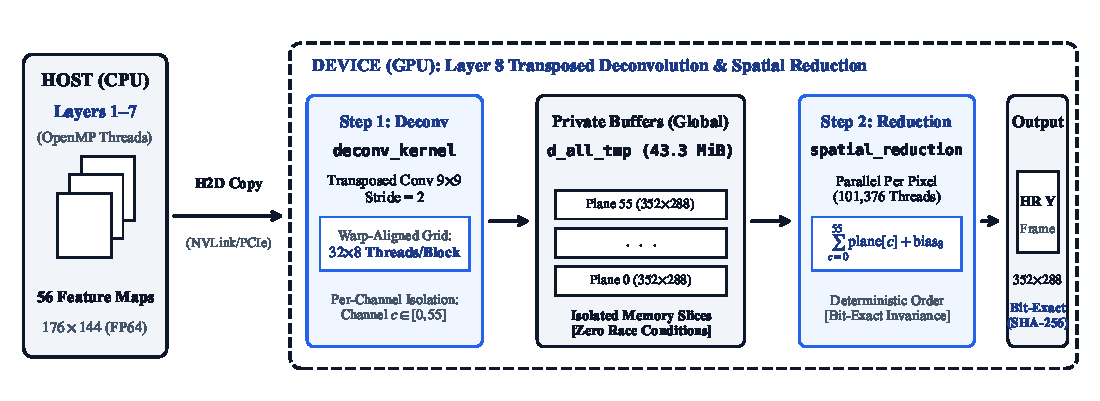
\includegraphics[width=0.92\textwidth]{figures/architecture_pipeline.pdf}
\caption{Architecture and execution workflow of the proposed GPU spatial reduction framework. Host CPU executes Layers 1--7 to generate 56 low-resolution feature maps ($176{\times}144$). The GPU \texttt{deconv\_kernel} computes the $9{\times}9$ transposed convolution using warp-aligned $32{\times}8$ thread blocks, writing isolated output planes into private device buffer \texttt{d\_all\_tmp} to eliminate write races by construction. Subsequently, \texttt{spatial\_reduction} executes a parallel channel reduction per output pixel in fixed order, guaranteeing bit-exact deterministic reconstruction.}
\label{fig:pipeline}
\end{figure*}

We implement Layer~8 via two custom CUDA kernels rather than relying on cuDNN~\cite{chetlur2014cudnn} or atomic accumulation (\texttt{atomicAdd}) (Fig.~\ref{fig:pipeline}). In floating-point arithmetic, addition is non-associative: $(a + b) + c \neq a + (b + c)$. Using \texttt{atomicAdd} across asynchronous warps produces non-deterministic summation orders depending on dynamic thread scheduling, introducing minor rounding divergences that destroy bit-exact reproducibility. Furthermore, black-box libraries such as cuDNN optimize for batched matrix multiplication without exposing the isolated per-channel intermediate buffers required by our zero-race verification contract. Custom kernels guarantee an invariant per-channel layout and deterministic summation order across runs and architectures.

\emph{Deconvolution kernel.} Each thread block processes a 2D tile of the input feature map. For each channel $c \in [0,55]$, threads compute the $9{\times}9$ transposed convolution and write into an isolated channel plane of \texttt{d\_all\_tmp}, indexed $c \times (H_{out}W_{out}) + yW_{out} + x$.

\emph{Spatial reduction kernel.} One thread per output pixel $(y,x)$ iterates all 56 planes, sums them, and adds the Layer~8 bias:
\begin{equation}
\text{output}[y, x] = \left( \sum_{c=0}^{55} \text{d\_all\_tmp}[c, y, x] \right) + \text{bias}_8
\label{eq:spatial_reduction}
\end{equation}
Channel writes are isolated during deconvolution and read-only during reduction, ensuring execution is race-free and deterministic by construction.

NVIDIA GPUs execute threads in SIMD groups of 32 called \emph{warps}~\cite{nvidiacudaguide}. A standard $16{\times}16$ block places only 16 threads along the row-major X dimension, splitting warps across non-contiguous rows. Because warp sizing governs SIMT throughput~\cite{lashgar2012warpresize}, we evaluate a $32{\times}8$ block (256 threads): setting $B_x=32$ guarantees all 32 threads in a warp access contiguous doubles along an image row, maximizing coalescing.

%%%%%%%%%%%%%%%%%%%%%%%%%%%%%%%%%%%%%%%%%%%%%%%%%%%%%%%%%%%%%%%%%%%%%%%%%%%%%%%
\section{Experimental Evaluation}

\subsection{Evaluation Methodology}
\label{sec:methodology}
The workload consists of 150 frames of the Suzie sequence ($176{\times}144 \rightarrow 352{\times}288$, YUV420p). Every configuration was executed 7 times: run 1 discarded as warmup, and runs 2--7 recorded as mean $\pm$ SD. CPU binaries use \texttt{gcc -fopenmp -O3} (default \texttt{libgomp} static scheduling); GPU binaries use \texttt{nvcc -O3 -arch=native}. Both platforms run GCC 13.3.0 and CUDA 13.0. All arithmetic is double precision, matching the CPU baseline to enable strict bit-exact comparison.

\emph{Reference file:} We execute single-threaded V1 once to generate a deterministic reference. Correctness is verified via byte comparison (\texttt{cmp -l}, $\text{diff\_bytes}=0$ between V1 and V2 across all grid configurations) and PSNR/SSIM~\cite{wang2004ssim} via \texttt{ffmpeg}; bit-exactness is reported when PSNR$=\infty$. Because untouched chroma inflates all-component averages, we report luminance-only values (PSNR-Y) wherever corruption severity is evaluated.

V0 degrades non-monotonically due to data races: $13.8$~dB on the GB10 (4 threads) and $68.6$~dB/$0.99996$ on the RTX 4090 (4 threads) before collapsing to $23.0$~dB at 32 threads. Although a $68.6$~dB error is imperceptible to visual inspection, it remains non-deterministic. Three consecutive V0 runs at 32 threads corrupted $4.75$, $5.01$, and $5.04$ million bytes ($21.34$, $21.46$, $21.63$~dB PSNR-Y), producing non-reproducible outputs. Fig.~\ref{fig:correctness} illustrates this degradation.

\begin{figure}[htbp]
\centering
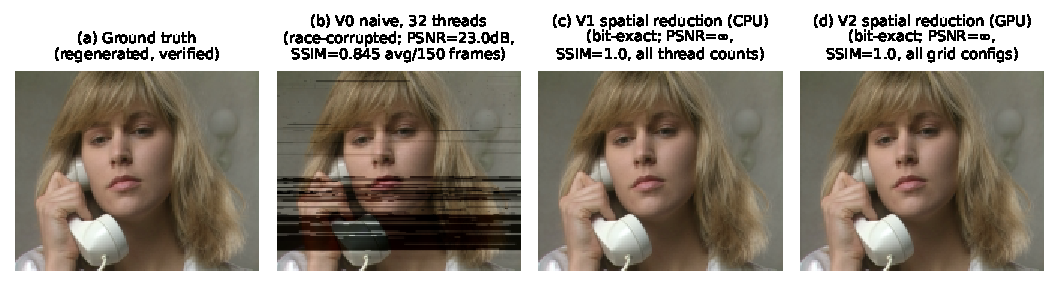
\includegraphics[width=0.88\columnwidth]{figures/correctness_visual_check.pdf}
\caption{Frame 26. (b) CPU-only naive baseline (V0, 32 threads on i9-14900K, $21.5$~dB PSNR-Y / $0.767$ SSIM against reference (a)), exhibiting scanline artifacts from concurrent writes to \texttt{img\_fltr\_8}. (c) CPU V1 and (d) GPU V2 are bit-identical to (a) across all configurations.}
\label{fig:correctness}
\end{figure}

\subsection{Performance Scaling \& Accuracy Benchmark}

Table~\ref{tab:benchmark} presents results for both platforms across thread counts, accuracy, and GPU grid configurations.

\begin{table*}[htbp]
\caption{Key Configurations on Both Platforms: Performance and Deviation from Each Platform's Verified Deterministic Reference. Wall times are mean $\pm$ SD over the 6 measured runs of a 7-run repetition.}
\label{tab:benchmark}
\centering
\footnotesize
\setlength{\tabcolsep}{3pt}
\resizebox{\textwidth}{!}{%
\begin{tabular}{llcccccc}
\toprule
Variant & Configuration / Threads & Wall Time (ms) & Speedup vs. Serial & Speedup vs. Best CPU & Dev. from Ref. (dB) & SSIM & GPU L8 Kernel (ms) \\
\midrule
\multicolumn{8}{l}{\emph{GB10 (ASUS GX10), unified memory; CPU thread ladder 1--20}} \\
CPU V0 (Naive) & 1 Thread & $18{,}240.50 \pm 228.82$ & 1.00$\times$ & N/A & bit-exact & bit-exact & N/A \\
CPU V0 (Naive) & 4 Threads (worst) & $7{,}074.33 \pm 90.21$ & 2.58$\times$ & N/A & 13.785 & 0.518246 & N/A \\
CPU V0 (Naive) & 20 Threads (Max, fastest) & $6{,}346.33 \pm 32.60$ & 2.87$\times$ & N/A & 25.751 & 0.838930 & N/A \\
CPU V1 (Baseline) & 1 Thread (Serial) & $21{,}552.33 \pm 298.07$ & 1.00$\times$ & N/A & bit-exact & bit-exact & N/A \\
CPU V1 & 4 Threads (cf. RTX optimum) & $8{,}316.50 \pm 58.06$ & 2.59$\times$ & N/A & bit-exact & bit-exact & N/A \\
CPU V1 (Max Cores) & 20 Threads (fastest verified) & $6{,}921.83 \pm 82.49$ & 3.11$\times$ & N/A & bit-exact & bit-exact & N/A \\
GPU V2 (Hybrid) & Grid $16{\times}16\_256$ (baseline) & $4{,}935.67 \pm 36.30$ & 4.37$\times$ & 1.40$\times$ & bit-exact & bit-exact & $696.51 \pm 1.78$ \\
GPU V2 (Best Grid) & Grid $32{\times}8\_256$ & $4{,}756.33 \pm 30.71$ & 4.53$\times$ & 1.46$\times$ & bit-exact & bit-exact & $533.19 \pm 2.58$ \\
\midrule
\multicolumn{8}{l}{\emph{RTX 4090 desktop, discrete memory; CPU thread ladder 1--32, 4-thread GPU backdrop}} \\
CPU V0 (Naive) & 1 Thread & $20{,}973.50 \pm 36.30$ & 1.00$\times$ & N/A & bit-exact & bit-exact & N/A \\
CPU V0 (Naive) & 4 Threads (fastest) & $8{,}207.67 \pm 247.16$ & 2.56$\times$ & N/A & 68.559 & 0.999957 & N/A \\
CPU V0 (Naive) & 32 Threads (Max, worst) & $26{,}388.67 \pm 664.00$ & 0.79$\times$ & N/A & 23.006 & 0.845283 & N/A \\
CPU V1 (Baseline) & 1 Thread (Serial) & $22{,}904.17 \pm 86.90$ & 1.00$\times$ & N/A & bit-exact & bit-exact & N/A \\
CPU V1 (Best) & 4 Threads (fastest verified) & $8{,}844.17 \pm 132.68$ & 2.59$\times$ & N/A & bit-exact & bit-exact & N/A \\
GPU V2 (Hybrid) & Grid $16{\times}16\_256$ (baseline) & $5{,}579.00 \pm 166.61$ & 4.11$\times$ & 1.59$\times$ & bit-exact & bit-exact & $437.06 \pm 3.86$ \\
GPU V2 (Best Grid) & Grid $32{\times}8\_256$ & $5{,}435.50 \pm 148.01$ & 4.21$\times$ & 1.63$\times$ & bit-exact & bit-exact & $360.92 \pm 7.22$ \\
\bottomrule
\end{tabular}%
}

\vspace{0.5ex}
\begin{minipage}{\textwidth}
\footnotesize
\emph{Speedup vs. Serial}: CPU against own 1-thread baseline; GPU V2 against CPU V1 serial. \emph{Speedup vs. Best CPU}: GPU V2 against CPU V1 fastest verified configuration. \emph{Dev./SSIM}: evaluated against platform-specific deterministic reference; ``bit-exact'' indicates $\text{diff\_bytes}=0$ and PSNR$=\infty$. \emph{GPU L8 Kernel}: mean $\pm$ SD across 6 profiled runs (Section~\ref{sec:breakdown}).
\end{minipage}
\end{table*}

\subsection{Reconstruction Quality Against a High-Resolution Reference}
\label{sec:quality}
To evaluate reconstruction quality against ground truth, the Suzie sequence was bicubic-downsampled ($88{\times}72$) and reconstructed at $2\times$ scale ($176{\times}144$). Evaluating the Y plane, FSRCNN achieves $37.86$~dB PSNR-Y and $0.9665$ SSIM-Y versus bicubic upscaling's $35.69$~dB and $0.9532$, a $+2.17$~dB gain confirming baseline quality fidelity.

\subsection{The Cost of Determinism, Quantified}
\label{sec:cost-of-determinism}
Table~\ref{tab:benchmark} quantifies the CPU determinism penalty via the wall-time delta between V0 (racy) and V1 (privatized): $+18.2\%$, $+17.6\%$, and $+9.1\%$ at 1, 4, and 20 threads on the GB10, and $+9.2\%$ and $+7.8\%$ at 1 and 4 threads on the RTX 4090. This overhead measures the cost of writing and re-reading $43.3$~MiB of private buffer space, amounting to $8$--$18\%$ of CPU wall time.

On the GPU, per-kernel instrumentation reveals that the reduction pass constitutes $4.6\%$ of Layer~8 execution time on the GB10 and only $0.6\%$ on the RTX 4090 (amounting to $0.55\%$ and $0.05\%$ of total wall time). Peak device allocation remains bounded at $44.3$~MiB ($<0.1\%$ of system memory). This divergence is architectural: the reduction is bandwidth-bound, and the RTX 4090's 72~MB L2 cache accommodates the entire working set, whereas the GB10 streams from unified DRAM near hardware peak. Determinism is thus near-free whenever the privatization buffer fits within last-level cache.

\subsection{Fine-Grained GPU Timing Breakdown}
\label{sec:breakdown}
We instrumented CUDA Event profiling inside the GPU binary across six runs of the optimal $32{\times}8\_256$ grid (Table~\ref{tab:breakdown}). The host counter \texttt{h2d\_ms} is excluded because blocking copies serialize behind draining kernels, charging execution latency to transfer; per-kernel event decomposition isolates actual execution.

\begin{table}[htbp]
\caption{Layer~8 Profiling Breakdown, $32{\times}8\_256$, 150 Frames (ms, mean $\pm$ SD over 6 runs)}
\label{tab:breakdown}
\centering
\resizebox{\columnwidth}{!}{%
\begin{tabular}{lrr}
\toprule
Pipeline Stage & GB10 (unified) & RTX 4090 (discrete) \\
\midrule
CPU Layers 1--7 & $3{,}392.82 \pm 21.62$ & $4{,}624.50 \pm 70.96$ \\
GPU Layer 8, event window & $533.19 \pm 2.58$ & $360.92 \pm 7.22$ \\
\quad$\hookrightarrow$ \texttt{deconv\_kernel} ($56\times$) & $424.07 \pm 0.76$ & $261.90 \pm 3.09$ \\
\quad$\hookrightarrow$ \texttt{spatial\_reduction} ($1\times$) & $26.32 \pm 1.02$ & $2.62 \pm 0.01$ \\
\quad$\hookrightarrow$ in-window transfer, gaps & $127.65 \pm 4.10$ & $152.14 \pm 0.36$ \\
Device-to-Host & $3.46 \pm 0.06$ & $16.42 \pm 0.49$ \\
Unaccounted (launch, file I/O) & $821.20$ & $469.33$ \\
\midrule
Total Wall Time & $4{,}750.67 \pm 30.40$ & $5{,}471.17 \pm 76.17$ \\
\bottomrule
\end{tabular}%
}

\vspace{0.5ex}
\begin{minipage}{\columnwidth}
\footnotesize
Indented rows decompose the event window. Instrumentation overhead ($5.34$~\textmu s on GB10, $6.64$~\textmu s on RTX 4090 per launch) inflates the window by $8.4\%$ and $15.4\%$, concentrated in the $8{,}400$ deconvolution launches. The reduction kernel ($150$ launches) incurs only $\sim$0.80~ms overhead.
\end{minipage}
\end{table}

Two findings stand out. First, the reduction kernel requires $26.32$~ms on the GB10 but only $2.62$~ms on the RTX 4090, a $10.0\times$ gap. Reading the $43.31$~MiB private buffer once per frame ($6.81$~GB total) represents $259$~GB/s on the GB10 ($95\%$ of its $273$~GB/s LPDDR5x peak~\cite{asusgx10_datasheet}) and $2{,}597$~GB/s effective bandwidth on the RTX 4090 ($2.5\times$ its $1{,}008$~GB/s GDDR6X ceiling). This confirms that the RTX 4090 serves the reduction primarily from its 72~MB L2 cache, whereas the GB10 streams from unified memory.

Second, device-to-host transfer exhibits the opposite pattern: $3.46$~ms on the GB10 versus $16.42$~ms on the RTX 4090 ($4.74\times$ faster on unified memory, $35.1$ vs. $7.4$~GB/s effective). Measured outside the event window after synchronization, this provides a clean demonstration of the unified-memory transfer advantage. Peak device memory remained constant at $44.3$~MiB across all configurations.

%%%%%%%%%%%%%%%%%%%%%%%%%%%%%%%%%%%%%%%%%%%%%%%%%%%%%%%%%%%%%%%%%%%%%%%%%%%%%%%
\section{Discussion and Key Insights}

\subsection{Speedup vs. Maxed-Out CPU Cores, and Warp Alignment}
\label{sec:gb10-speedup}
We evaluate speedup against CPU V1 because V1 guarantees race-free execution across all thread counts, whereas V0 is only incidentally correct at 1 thread. Although V0 yields a faster wall time at 20 threads ($6{,}346.33$~ms, implying a $1.33\times$ speedup), its output is corrupted. GPU V2 ($32{\times}8\_256$) reaches $4{,}756.33$~ms ($31.5$ FPS), achieving a $1.46\times$ speedup over CPU V1's fastest verified configuration ($6{,}921.83$~ms at 20 threads).

At 1 thread, V0 is bit-exact and faster than V1 ($18{,}240.50$ vs. $21{,}552.33$~ms) by avoiding privatization overhead, providing the fastest bit-exact serial baseline: GPU V2 achieves $3.84\times$ (GB10) and $3.86\times$ (RTX 4090) speedups. The GB10's ARM big.LITTLE cores scale smoothly across the 20-thread ladder~\cite{wang2020pipeit}, avoiding the high-thread degradation observed on the discrete desktop.

Transitioning from the default $16{\times}16$ grid ($696.51 \pm 1.78$~ms) to the warp-aligned $32{\times}8$ grid ($533.19 \pm 2.58$~ms) reduces kernel time by $23.4\%$ (Welch's $t = -127.50$, $df = 8.9$, $p < 10^{-4}$). This gain stems from memory coalescing: a 32-thread row width aligns warp accesses to contiguous memory. Because block sizing alters only the 2D deconvolution, the speedup is confined entirely to \texttt{deconv\_kernel} (dropping $24.9\%$ from $564.74$ to $424.07$~ms), while the reduction kernel remains constant ($26.08$ vs. $26.32$~ms).

\subsection{Transfer Cost and Amdahl's Law}
\label{sec:nvlink}
Data transfer is not a bottleneck on either platform. On the GB10, the non-kernel event window residual totals $127.65$~ms ($2.7\%$ of wall time), with D2H copy adding $3.46$~ms; even assigning the entire residual to transfer bounds total transfer overhead below $3\%$. The RTX 4090 incurs a larger residual ($152.14$~ms, $36.5\%$ of its window), consistent with PCIe latency.

Table~\ref{tab:breakdown} highlights an Amdahl's Law~\cite{amdahl1967} ceiling: Layer~8 accounts for only $11.2\%$ (GB10) and $6.6\%$ (RTX 4090) of wall time, whereas CPU Layers 1--7 consume $71.4\%$ and $84.5\%$. Eliminating Layer~8 entirely would leave total pipeline time above $88\%$, indicating that offloading Layers 1--7 is essential for sub-second reconstruction.

%%%%%%%%%%%%%%%%%%%%%%%%%%%%%%%%%%%%%%%%%%%%%%%%%%%%%%%%%%%%%%%%%%%%%%%%%%%%%%%
\section{Cross-Platform Validation on Discrete-GPU Hardware}
\label{sec:rtx4090}

We replicated the evaluation on an Intel Core i9-14900K desktop with an RTX 4090 (Table~\ref{tab:hardware}), featuring separate PCIe memory and hybrid P/E-core CPU architecture.

\subsection{Methodology Adjustment and GPU Speedup}
On the hybrid CPU, wall time collapses past 8 threads ($\sim$3.5$\times$ slowdown relative to 4 threads), consistent with asymmetric core contention without explicit OpenMP thread affinity~\cite{eichenberger2012ompaffinity}. Using the platform's optimal 4-thread CPU backdrop, GPU V2 achieves $5{,}435$--$5{,}579$~ms ($26.9$--$27.6$ FPS), representing a $1.59\times$--$1.63\times$ speedup over CPU V1's fastest configuration ($8{,}844.17$~ms).

\subsection{Cross-Architecture Bit-Exactness}
\label{sec:cross-arch-bitexact}
Comparing outputs across platforms addresses a stringent determinism test. The GB10 (ARM host, Blackwell \texttt{sm\_121}) and RTX 4090 (x86 host, Ada \texttt{sm\_89}) differ in host ISA and GPU architecture. Across identical runs, \texttt{cmp -l} confirms 0 differing bytes, and SHA-256 digests match bit-for-bit (\texttt{8db2c07a...ca066b}), proving invariant cross-platform reproducibility.

\subsection{Warp Alignment Generalizes Across GPU Architectures}
\label{sec:warp-generalize}
The $32{\times}8$ block remains fastest on Ada Lovelace ($360.92 \pm 7.22$~ms vs. $437.06 \pm 3.86$~ms for $16{\times}16$, a $17.4\%$ reduction; Welch's $t = -22.77$, $df = 7.6$, $p < 10^{-4}$). The gain isolates to \texttt{deconv\_kernel} ($15.6\%$ reduction), while the reduction remains fixed at $2.62$~ms (Fig.~\ref{fig:warp-cross}).

\begin{figure}[htbp]
\centering
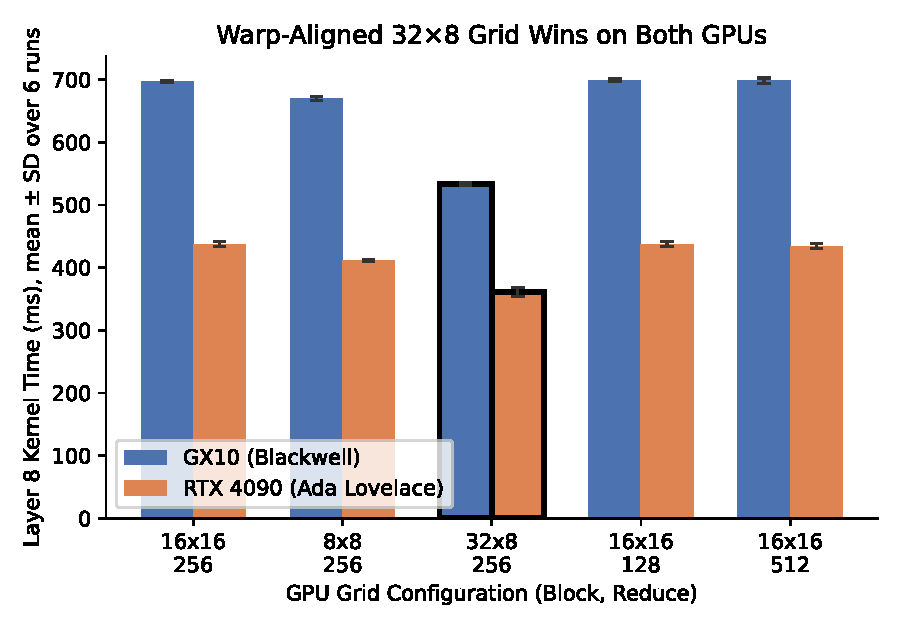
\includegraphics[width=0.88\columnwidth]{figures/warp_alignment_cross_platform.pdf}
\caption{GPU Layer~8 kernel time across grid configurations (mean $\pm$ SD over 6 runs). The warp-aligned $32{\times}8$ grid is fastest across both architectures.}
\label{fig:warp-cross}
\end{figure}

\subsection{Non-Unified Memory and FP64 Precision}
Despite discrete PCIe transfers, the RTX 4090 achieves faster Layer~8 kernel times due to higher compute capacity and its 72~MB L2 cache. Furthermore, because Ada Lovelace restricts FP64 throughput to $1/64$ of FP32, the GPU operates with most compute units underutilized; an FP32 pipeline would yield substantially higher throughput at the cost of strict bit-exact determinism.

%%%%%%%%%%%%%%%%%%%%%%%%%%%%%%%%%%%%%%%%%%%%%%%%%%%%%%%%%%%%%%%%%%%%%%%%%%%%%%%
\section{Limitations and Future Work}
\label{sec:limitations}
Several limitations bound this study, each with a concrete next step. First, competitive baselines such as \texttt{atomicAdd} and cuDNN were omitted because non-associative floating-point addition across asynchronous warps breaks bit-exactness, and closed-source cuDNN routines do not expose the per-channel buffers our verification depends on; a throughput-only comparison against both is still useful future work to price determinism against an unconstrained baseline. Second, our L2 residency model is inferred from bandwidth arithmetic rather than measured directly: the next step is Nsight Compute profiling of L2 hit rate and memory throughput on both GPUs to confirm it with hardware counters. Third, host-to-device measurements include launch latency and host padding. Fourth, we evaluated one 150-frame QCIF-to-CIF Suzie sequence ($176{\times}144 \rightarrow 352{\times}288$) at one scale factor for direct comparability with~\cite{annisa2025}; scaling to 1080p and 4K at $2\times$ and $4\times$ would push the working set past the RTX 4090's 72~MB L2 cache and test the cache-overflow threshold directly, and additional sequences would separate content-dependent effects from the architectural ones reported here. Finally, an FP32 or mixed FP16/BF16 variant of Layer~8 is the natural next experiment: it would put a number on what bit-exact determinism costs in throughput, the trade this paper argues for but does not measure.

%%%%%%%%%%%%%%%%%%%%%%%%%%%%%%%%%%%%%%%%%%%%%%%%%%%%%%%%%%%%%%%%%%%%%%%%%%%%%%%
\section{Conclusion}
We presented a GPU spatial-reduction framework for FSRCNN's deconvolution layer, eliminating multi-threaded write races by construction. Evaluated across unified (GB10) and discrete (RTX 4090) platforms, our approach guarantees bit-exact output matching a deterministic CPU reference across all configurations, as well as bit-identical cross-platform reproducibility spanning two host ISAs and GPU generations. Warp-aligned $32{\times}8$ blocks optimize memory coalescing, accelerating deconvolution by $23.4\%$ and $17.4\%$, and yielding speedups of $1.46\times$ ($31.5$ FPS) and $1.63\times$ ($27.6$ FPS) over verified multicore CPU baselines. Platform asymmetries reveal that unified memory delivers $4.74\times$ faster host-device transfers, while discrete GPUs accelerate the bandwidth-bound reduction tenfold when intermediate buffers fit within last-level cache.

%%%%%%%%%%%%%%%%%%%%%%%%%%%%%%%%%%%%%%%%%%%%%%%%%%%%%%%%%%%%%%%%%%%%%%%%%%%%%%%
\begin{thebibliography}{00}
\footnotesize
\setlength{\itemsep}{0pt plus 0.2pt}

\bibitem{annisa2025} A. Annisa, A. Adnan, and Z. Zainuddin, ``Enhancing computational efficiency: Transitioning from serial to parallel programming for low-to-high resolution video reconstruction using FSRCNN on AMP architecture,'' in \emph{Proc. IEEE Int. Conf. Artif. Intell. Mechatron. Syst. (AIMS)}, 2025, pp. 1--8.

\bibitem{dong2016fsrcnn} C. Dong, C. C. Loy, and X. Tang, ``Accelerating the super-resolution convolutional neural network,'' in \emph{Proc. ECCV}, 2016, pp. 391--407.

\bibitem{wang2020pipeit} S. Wang, G. Ananthanarayanan, Y. Zeng, N. Goel, A. Pathania, and T. Mitra, ``High-throughput CNN inference on embedded ARM big.LITTLE multicore processors,'' \emph{IEEE Trans. Comput.-Aided Design Integr. Circuits Syst.}, vol. 39, no. 10, pp. 2254--2267, Oct. 2020.

\bibitem{bilbao2023pmcsched} C. Bilbao, J. C. Saez, and M. Prieto-Mat\'ias, ``Flexible system software scheduling for asymmetric multicore systems with PMCSched: A case for Intel Alder Lake,'' \emph{Concurr. Comput. Pract. Exper.}, vol. 35, no. 25, e7814, 2023.

\bibitem{eichenberger2012ompaffinity} A. E. Eichenberger, C. Terboven, M. Wong, and D. an Mey, ``The design of OpenMP thread affinity,'' in \emph{Proc. IWOMP}, LNCS 7312, 2012, pp. 15--28.

\bibitem{nvidiacudaguide} NVIDIA Corp., ``CUDA C++ programming guide,'' 2024. [Online]. Available: \url{https://docs.nvidia.com/cuda/cuda-c-programming-guide/}

\bibitem{go2017apunet} Y. Go, M. A. Jamshed, Y. Moon, C. Hwang, and K. Park, ``APUNet: Revitalizing GPU as packet processing accelerator,'' in \emph{Proc. USENIX NSDI}, 2017, pp. 83--96.

\bibitem{wang2004ssim} Z. Wang, A. C. Bovik, H. R. Sheikh, and E. P. Simoncelli, ``Image quality assessment: From error visibility to structural similarity,'' \emph{IEEE Trans. Image Process.}, vol. 13, no. 4, pp. 600--612, Apr. 2004.

\bibitem{dong2014srcnn} C. Dong, C. C. Loy, K. He, and X. Tang, ``Learning a deep convolutional network for image super-resolution,'' in \emph{Proc. ECCV}, 2014, pp. 184--199.

\bibitem{amdahl1967} G. M. Amdahl, ``Validity of the single processor approach to achieving large scale computing capabilities,'' in \emph{Proc. AFIPS}, 1967, pp. 483--485.

\bibitem{williams2009roofline} S. Williams, A. Waterman, and D. Patterson, ``Roofline: An insightful visual performance model for multicore architectures,'' \emph{Commun. ACM}, vol. 52, no. 4, pp. 65--76, Apr. 2009.

\bibitem{chetlur2014cudnn} S. Chetlur \emph{et al.}, ``cuDNN: Efficient primitives for deep learning,'' 2014, arXiv:1410.0759. [Online]. Available: \url{https://arxiv.org/abs/1410.0759}

\bibitem{serebryany2009threadsanitizer} K. Serebryany and T. Iskhodzhanov, ``ThreadSanitizer: Data race detection in practice,'' in \emph{Proc. WBIA}, 2009, pp. 62--71.

\bibitem{lashgar2012warpresize} A. Lashgar, A. Baniasadi, and A. Khonsari, ``Warp size impact in GPUs: Large or small?,'' in \emph{Proc. GPGPU-5}, 2012, pp. 27--32.

\bibitem{dumoulin2016convolution} V. Dumoulin and F. Visin, ``A guide to convolution arithmetic for deep learning,'' 2016, arXiv:1603.07285. [Online]. Available: \url{https://arxiv.org/abs/1603.07285}

\bibitem{nvidiagb10_2025} NVIDIA Corp., ``NVIDIA puts Grace Blackwell on every desk and at every AI developer's fingertips,'' NVIDIA Newsroom, Jan. 2025. [Online]. Available: \url{https://nvidianews.nvidia.com/news/nvidia-puts-grace-blackwell-on-every-desk-and-at-every-ai-developers-fingertips}

\bibitem{asusgx10_datasheet} ASUSTeK Computer Inc., \emph{ASUS Ascent GX10 Datasheet}, v8, 2025. [Online]. Available: \url{https://dlcdnwebimgs.asus.com/files/media/202506/5c0fb57c-4e48-4e96-8c97-04bf8df2677c/asus-ascent-gx10-datasheet.pdf}

\bibitem{armdynamiq} Arm Ltd., ``DynamIQ technology,'' 2024. [Online]. Available: \url{https://www.arm.com/technologies/dynamiq}

\bibitem{nvidiaada2022} NVIDIA Corp., ``NVIDIA Ada GPU architecture,'' Whitepaper V2.02, 2022.

\bibitem{nvidiagracehopper2022} NVIDIA Corp., ``Grace Hopper Superchip architecture in-depth,'' NVIDIA Developer Blog, 2022. [Online]. Available: \url{https://developer.nvidia.com/blog/nvidia-grace-hopper-superchip-architecture-in-depth/}

\bibitem{wahlgren2025upm} J. Wahlgren \emph{et al.}, ``Dissecting CPU-GPU unified physical memory on AMD MI300A APUs,'' in \emph{Proc. IEEE IISWC}, 2025.

\bibitem{chen2018tvm} T. Chen, T. Moreau, Z. Jiang, L. Zheng, E. Yan, H. Shen, M. Cowan, L. Wang, Y. Hu, L. Ceze, C. Guestrin, and A. Krishnamurthy, ``TVM: An automated end-to-end optimizing compiler for deep learning,'' in \emph{Proc. 13th USENIX Symp. Operating Syst. Des. Implement. (OSDI)}, Carlsbad, CA, 2018, pp. 578--594.

\bibitem{nvidiatensorrt} NVIDIA Corp., ``TensorRT: Architecture overview,'' 2025. [Online]. Available: \url{https://docs.nvidia.com/deeplearning/tensorrt/latest/architecture/architecture-overview.html}

\end{thebibliography}

\end{document}